\documentclass[12pt, a4paper]{article}

\usepackage{amsmath, amssymb, amsthm}
\usepackage{geometry}
\usepackage{hyperref}
\usepackage{booktabs}
\usepackage{array}
\usepackage{xcolor}
\usepackage{tikz}
\usepackage{mdframed}
\usepackage{enumitem}
\usepackage{parskip}
\usepackage{titlesec}

\geometry{margin=2.5cm}

\hypersetup{
    colorlinks=true,
    linkcolor=blue!70!black,
    urlcolor=blue!70!black
}

\definecolor{boxbg}{RGB}{240, 246, 255}
\definecolor{boxborder}{RGB}{70, 130, 200}

\newmdenv[
  backgroundcolor=boxbg,
  linecolor=boxborder,
  linewidth=1.5pt,
  roundcorner=5pt,
  innertopmargin=8pt,
  innerbottommargin=8pt,
  innerleftmargin=12pt,
  innerrightmargin=12pt
]{keybox}

\theoremstyle{definition}
\newtheorem{definition}{Definition}
\newtheorem{theorem}{Theorem}
\newtheorem*{remark}{Remark}

\titleformat{\section}{\large\bfseries\color{blue!70!black}}{{\thesection}}{1em}{}
\titleformat{\subsection}{\normalsize\bfseries}{{\thesubsection}}{1em}{}

\title{
    \vspace{-1cm}
    {\Large \textbf{The Moore--Penrose Pseudoinverse}}\\[0.4em]
    {\large Foundations, Derivations, and Connection to SVD}
}
\author{}
\date{\today}

\begin{document}

\maketitle
\tableofcontents
\newpage

% ─────────────────────────────────────────────
\section{Motivation}

A fundamental problem in linear algebra is solving the system
\[
    A\mathbf{x} = \mathbf{b}
\]
When $A \in \mathbb{R}^{n \times n}$ is square and invertible, the unique solution is $\mathbf{x} = A^{-1}\mathbf{b}$.
However, in many practical settings:

\begin{itemize}
    \item $A$ is \textbf{rectangular} (more equations than unknowns, or vice versa), so no square inverse exists.
    \item $A$ is \textbf{rank-deficient}, making it singular even if square.
    \item The system is \textbf{overdetermined} (no exact solution) or \textbf{underdetermined} (infinitely many solutions).
\end{itemize}

The \textbf{Moore--Penrose pseudoinverse} $A^+$ generalises the matrix inverse to handle all these cases gracefully.

% ─────────────────────────────────────────────
\section{Definition: The Moore--Penrose Conditions}

\begin{definition}
For $A \in \mathbb{R}^{m \times n}$, the \textbf{Moore--Penrose pseudoinverse} $A^+ \in \mathbb{R}^{n \times m}$ is the unique matrix satisfying all four Penrose conditions:
\begin{align}
    A A^+ A &= A \label{eq:p1}\\
    A^+ A A^+ &= A^+ \label{eq:p2}\\
    (A A^+)^\top &= A A^+ \label{eq:p3}\\
    (A^+ A)^\top &= A^+ A \label{eq:p4}
\end{align}
\end{definition}

Conditions \eqref{eq:p1} and \eqref{eq:p2} say $A^+$ acts as a ``weak'' two-sided inverse. Conditions \eqref{eq:p3} and \eqref{eq:p4} require the products $AA^+$ and $A^+A$ to be symmetric. Note that \eqref{eq:p1} already makes both products idempotent — e.g.\ $(AA^+)(AA^+) = (AA^+A)A^+ = AA^+$ — so they are always projectors; \eqref{eq:p3} and \eqref{eq:p4} upgrade them from oblique projectors to \emph{orthogonal} ones.

The definition quietly asserts uniqueness, which deserves proof — the argument, a pleasant exercise in using all four conditions, is given in Appendix~\ref{app:proofs}.

\begin{theorem}[Uniqueness]
\label{thm:uniqueness}
At most one matrix satisfies conditions \eqref{eq:p1}--\eqref{eq:p4}.
\end{theorem}

Existence is settled constructively in the next section: the SVD formula satisfies all four conditions.

\begin{keybox}
\textbf{Key fact:} When $A$ is square and invertible, $A^+ = A^{-1}$ recovers the ordinary inverse.
\end{keybox}

% ─────────────────────────────────────────────
\section{Connection to Singular Value Decomposition (SVD)}

\subsection{The SVD Factorisation}

Any matrix $A \in \mathbb{R}^{m \times n}$ of rank $r$ can be decomposed as:
\[
    A = U \Sigma V^\top
\]
where:
\begin{itemize}
    \item $U \in \mathbb{R}^{m \times m}$ — orthogonal matrix of \textbf{left singular vectors} (columns form an orthonormal basis for $\mathbb{R}^m$)
    \item $\Sigma \in \mathbb{R}^{m \times n}$ — diagonal matrix of \textbf{singular values} $\sigma_1 \geq \sigma_2 \geq \cdots \geq \sigma_r > 0$, with zeros elsewhere
    \item $V \in \mathbb{R}^{n \times n}$ — orthogonal matrix of \textbf{right singular vectors} (columns form an orthonormal basis for $\mathbb{R}^n$)
\end{itemize}

Since $U$ and $V$ are orthogonal, $U^{-1} = U^\top$ and $V^{-1} = V^\top$, making them cheap to invert.

\subsection{Geometric Picture: The Unit Sphere Becomes an Ellipse}

The factorisation $A = U\Sigma V^\top$ has a clean geometric reading: \textbf{every matrix maps the unit sphere to an ellipsoid.} Following the sphere through each factor, right to left:

\begin{enumerate}
    \item $V^\top$ is orthogonal, so it \textbf{rotates} the unit sphere rigidly onto itself — it just re-labels the sphere's surface so that the right singular vectors $\mathbf{v}_i$ land on the standard axes.
    \item $\Sigma$ then \textbf{scales} along each axis by $\sigma_i$, deforming the sphere into an axis-aligned ellipsoid with semi-axis lengths $\sigma_1, \ldots, \sigma_n$.
    \item $U$ is orthogonal too, so it \textbf{rotates} this ellipsoid rigidly into its final orientation, without changing its shape.
\end{enumerate}

The net effect: $A$ sends the unit sphere $\{\mathbf{x} : \|\mathbf{x}\| = 1\}$ to an ellipsoid whose semi-axes have lengths exactly the singular values $\sigma_i$, pointing along the left singular vectors $\mathbf{u}_i$. Concretely, each right singular vector maps directly to a semi-axis of the ellipsoid:
\[
    A\mathbf{v}_i = \sigma_i \mathbf{u}_i
\]

\begin{center}
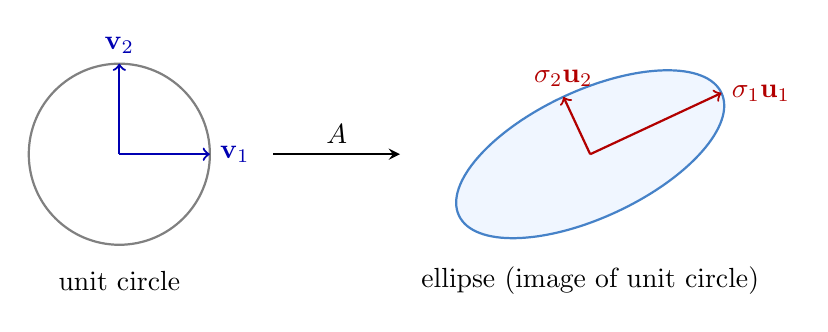
\begin{tikzpicture}[scale=1.15]
    % Unit circle
    \draw[thick, gray] (0,0) circle (1);
    \draw[thick, ->, blue!70!black] (0,0) -- (1,0) node[right] {$\mathbf{v}_1$};
    \draw[thick, ->, blue!70!black] (0,0) -- (0,1) node[above] {$\mathbf{v}_2$};
    \node at (0,-1.4) {unit circle};

    % Arrow with label
    \draw[thick, ->, >=stealth] (1.7,0) -- (3.1,0) node[midway, above] {$A$};

    % Ellipse (rotated)
    \begin{scope}[shift={(5.2,0)}, rotate=25]
        \draw[thick, boxborder, fill=boxbg] (0,0) ellipse (1.6 and 0.7);
        \draw[thick, ->, red!70!black] (0,0) -- (1.6,0) node[right] {$\sigma_1\mathbf{u}_1$};
        \draw[thick, ->, red!70!black] (0,0) -- (0,0.7) node[above] {$\sigma_2\mathbf{u}_2$};
    \end{scope}
    \node at (5.2,-1.4) {ellipse (image of unit circle)};
\end{tikzpicture}
\end{center}

This picture makes the pseudoinverse's job visually obvious: $A^+ = V\Sigma^+U^\top$ undoes exactly this deformation. It rotates the ellipsoid back so its axes align with $\mathbf{u}_i$, \textbf{shrinks} each axis by $1/\sigma_i$ (turning it back into a sphere), and rotates once more to land on the $\mathbf{v}_i$ directions. The largest singular value $\sigma_1$ is the sphere's most-stretched direction — and correspondingly the \emph{most-shrunk} direction under $A^+$, since $A^+$ divides by it.

\begin{keybox}
\textbf{Key fact:} A rank-deficient direction ($\sigma_i = 0$) is one the ellipsoid collapses completely flat along — that direction contributes zero thickness to the image, which is exactly why $\Sigma^+$ cannot invert it and instead sets $1/\sigma_i \to 0$.
\end{keybox}

\subsection{The Dual Picture: Which Shapes Map to a Circle?}

It is natural to ask the reverse question: what must a set look like in the \emph{input} space so that $A$ maps it exactly onto the unit sphere of the output space? If $A$ stretches each singular direction by $\sigma_i$, then a set destined to land on the sphere must be pre-shrunk by $1/\sigma_i$ along those same directions. Indeed, writing $\mathbf{x} = \sum_i c_i \mathbf{v}_i$ and using $A\mathbf{v}_i = \sigma_i\mathbf{u}_i$:
\[
    \|A\mathbf{x}\|^2 = \sum_i (\sigma_i c_i)^2 = 1
    \quad\Longleftrightarrow\quad
    \mathbf{x} \in \text{ellipsoid with semi-axes } \tfrac{1}{\sigma_i}\mathbf{v}_i
\]
(taking $A$ invertible for the moment). Note the inversion: the direction $A$ stretches \emph{most}, $\mathbf{v}_1$, is this ellipsoid's \emph{shortest} axis — a point there only needs to start $1/\sigma_1$ from the origin to land at distance one.

\begin{center}
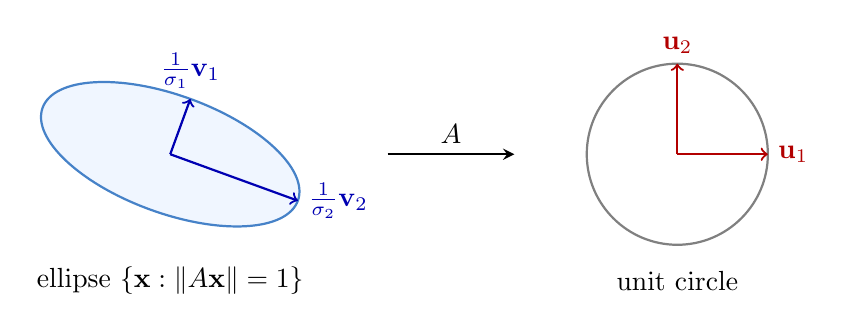
\begin{tikzpicture}[scale=1.15]
    % Input ellipse (long axis along v2 since 1/sigma_2 > 1/sigma_1)
    \begin{scope}[rotate=-20]
        \draw[thick, boxborder, fill=boxbg] (0,0) ellipse (1.5 and 0.65);
        \draw[thick, ->, blue!70!black] (0,0) -- (1.5,0) node[right] {$\tfrac{1}{\sigma_2}\mathbf{v}_2$};
        \draw[thick, ->, blue!70!black] (0,0) -- (0,0.65) node[above] {$\tfrac{1}{\sigma_1}\mathbf{v}_1$};
    \end{scope}
    \node at (0,-1.4) {ellipse $\{\mathbf{x} : \|A\mathbf{x}\| = 1\}$};

    % Arrow with label
    \draw[thick, ->, >=stealth] (2.4,0) -- (3.8,0) node[midway, above] {$A$};

    % Unit circle output
    \begin{scope}[shift={(5.6,0)}]
        \draw[thick, gray] (0,0) circle (1);
        \draw[thick, ->, red!70!black] (0,0) -- (1,0) node[right] {$\mathbf{u}_1$};
        \draw[thick, ->, red!70!black] (0,0) -- (0,1) node[above] {$\mathbf{u}_2$};
    \end{scope}
    \node at (5.6,-1.4) {unit circle};
\end{tikzpicture}
\end{center}

The punchline: this input ellipsoid is exactly the \textbf{image of the unit sphere under $A^+$}. This is immediate from the SVD — $A^+ = V\Sigma^+U^\top$ is itself an SVD-style factorisation with singular values $1/\sigma_i$ and the roles of $\mathbf{u}_i, \mathbf{v}_i$ swapped, so $A^+$ sends the unit sphere to the ellipsoid with semi-axes $\tfrac{1}{\sigma_i}\mathbf{v}_i$.

\begin{keybox}
\textbf{Duality.} $A$ maps the unit sphere to the ellipsoid with semi-axes $\sigma_i\mathbf{u}_i$; $A^+$ maps the unit sphere to the ellipsoid with semi-axes $\tfrac{1}{\sigma_i}\mathbf{v}_i$. Each map's output ellipsoid is precisely the set the \emph{other} map carries onto the unit sphere. For invertible $A$ this is just the statement $A^+ = A^{-1}$ in geometric form.
\end{keybox}

When $A$ is rank-deficient the picture degenerates consistently in both spaces. In the input space, motion along $\text{null}(A)$ is invisible to $A$, so $\{\mathbf{x} : \|A\mathbf{x}\| = 1\}$ becomes an elliptical \emph{cylinder} (the ellipse extruded freely along the null space) — and it reaches only the part of the unit sphere lying in $\text{col}(A)$. Correspondingly, $A^+$'s unit-sphere image gains no axis in those directions: $\Sigma^+$ puts a $0$ where $1/\sigma_i$ would blow up, flattening the ellipsoid instead of extruding it. The pseudoinverse resolves both ambiguities the same way — by ignoring the directions that carry no information.

\subsection{Full vs.\ Thin SVD}

\begin{center}
\renewcommand{\arraystretch}{1.4}
\begin{tabular}{lccc}
    \toprule
    & $U$ & $\Sigma$ & $V$ \\
    \midrule
    \textbf{Full SVD} & $m \times m$ & $m \times n$ & $n \times n$ \\
    \textbf{Thin SVD} & $m \times r$ & $r \times r$ & $n \times r$ \\
    \bottomrule
\end{tabular}
\end{center}

For computing $A^+$, the \textbf{thin SVD} is sufficient — the extra columns in the full SVD correspond to zero singular values and contribute nothing.

\subsection{The Pseudoinverse via SVD}

\begin{theorem}
\label{thm:svd}
Given $A = U\Sigma V^\top$, the Moore--Penrose pseudoinverse is:
\[
    \boxed{A^+ = V \Sigma^+ U^\top}
\]
where $\Sigma^+ \in \mathbb{R}^{n \times m}$ is the \emph{transpose} of $\Sigma$ with each non-zero singular value replaced by its reciprocal (zeros stay zero):
\[
    \Sigma^+ = \operatorname{diag}\!\left(\frac{1}{\sigma_1},\, \frac{1}{\sigma_2},\, \ldots,\, \frac{1}{\sigma_r},\, 0,\, \ldots,\, 0\right) \in \mathbb{R}^{n \times m}
\]
\end{theorem}

The proof — a direct verification of the four Penrose conditions, in which the orthogonality of $U$ and $V$ does all the work — is given in Appendix~\ref{app:proofs}. Combined with Theorem~\ref{thm:uniqueness}, it also settles existence: since every matrix has an SVD, every matrix has a pseudoinverse.

\textbf{Intuition.} SVD says: rotate ($V^\top$) $\to$ scale ($\Sigma$) $\to$ rotate ($U$). The pseudoinverse simply reverses this: rotate back ($U^\top$) $\to$ invert the scaling ($\Sigma^+$) $\to$ rotate back ($V$). The orthonormality of $U$ and $V$ makes this clean reversal possible.

\textbf{Why zeros stay zero.} Rank-deficient directions (zero singular values) carry no information about $A$ — they correspond to the null space. Trying to invert them would be division by zero, and setting them to zero is exactly what discards these redundant directions, mirroring the intuition of ``removing linearly dependent columns.''

% ─────────────────────────────────────────────
\section{Three Regimes: Square, Tall, and Wide Matrices}

\subsection{Square, Full-Rank Matrix}

$A \in \mathbb{R}^{n \times n}$, rank $n$. A unique exact solution exists:
\[
    \mathbf{x} = A^{-1}\mathbf{b} = A^+\mathbf{b}
\]

\subsection{Tall Matrix: Overdetermined System}

$A \in \mathbb{R}^{m \times n}$ with $m > n$, full column rank. More equations than unknowns — no exact solution in general. The pseudoinverse gives the \textbf{least-squares solution}:
\[
    \mathbf{x}^+ = A^+\mathbf{b} = (A^\top A)^{-1} A^\top \mathbf{b}
    \qquad \text{minimises } \|A\mathbf{x} - \mathbf{b}\|^2
\]

\subsection{Wide Matrix: Underdetermined System}

$A \in \mathbb{R}^{m \times n}$ with $m < n$, full row rank. More unknowns than equations — infinitely many exact solutions exist. The pseudoinverse gives the \textbf{minimum-norm solution}:
\[
    \mathbf{x}^+ = A^+\mathbf{b} = A^\top(AA^\top)^{-1}\mathbf{b}
    \qquad \text{minimises } \|\mathbf{x}\|
\]

\begin{center}
\renewcommand{\arraystretch}{1.5}
\begin{tabular}{lcccc}
    \toprule
    \textbf{Case} & \textbf{Shape} & \textbf{Solutions} & \textbf{$A^+$ formula} & \textbf{Minimises} \\
    \midrule
    Square (full rank) & $n \times n$ & Exactly one & $A^{-1}$ & --- \\
    Tall (full col rank) & $m \times n$, $m > n$ & None (exact) & $(A^\top A)^{-1}A^\top$ & $\|A\mathbf{x}-\mathbf{b}\|$ \\
    Wide (full row rank) & $m \times n$, $m < n$ & Infinitely many & $A^\top(AA^\top)^{-1}$ & $\|\mathbf{x}\|$ \\
    Rank-deficient & Any & None or $\infty$ & $V\Sigma^+U^\top$ & Both \\
    \bottomrule
\end{tabular}
\end{center}

All four rows are instances of a single statement:

\begin{theorem}[Minimum-norm least-squares solution]
For any $A \in \mathbb{R}^{m \times n}$ and $\mathbf{b} \in \mathbb{R}^m$, the vector $\mathbf{x}^+ = A^+\mathbf{b}$ is the unique solution of
\[
    \min_{\mathbf{x}}\; \|\mathbf{x}\| \quad \text{subject to} \quad \|A\mathbf{x} - \mathbf{b}\| = \min_{\mathbf{z}}\, \|A\mathbf{z} - \mathbf{b}\|.
\]
\end{theorem}

In words: among all least-squares minimisers — there may be exactly one, or an affine family of them — $A^+\mathbf{b}$ is the shortest. When exact solutions exist, the least-squares constraint is vacuous and only minimality of $\|\mathbf{x}\|$ bites (the wide case); when the minimiser is unique, minimality of $\|\mathbf{x}\|$ is vacuous instead (the square and tall cases); in the rank-deficient case both are active at once.

% ─────────────────────────────────────────────
\section{Derivations of the Pseudoinverse (Tall Case)}

We focus on the tall, full-column-rank case where $A^+ = (A^\top A)^{-1}A^\top$.

\subsection{Derivation 1: Least Squares (Calculus)}

\textbf{Goal:} Minimise $f(\mathbf{x}) = \|A\mathbf{x} - \mathbf{b}\|^2$.

Expanding:
\[
    f(\mathbf{x}) = \mathbf{x}^\top A^\top A \mathbf{x} - 2\mathbf{x}^\top A^\top \mathbf{b} + \mathbf{b}^\top \mathbf{b}
\]
Differentiating and setting to zero:
\[
    \nabla_{\mathbf{x}} f = 2A^\top(A\mathbf{x} - \mathbf{b}) = \mathbf{0}
\]
This yields the \textbf{normal equations}:
\[
    A^\top A \mathbf{x} = A^\top \mathbf{b}
\]
Since $A$ has full column rank, $A^\top A$ is $n \times n$ and invertible. Solving:
\[
    \mathbf{x}^+ = (A^\top A)^{-1} A^\top \mathbf{b} \implies A^+ = (A^\top A)^{-1} A^\top
\]

\subsection{Derivation 2: Geometric Projection}

\textbf{Column space perspective.} When $A\mathbf{x} = \mathbf{b}$ has no exact solution, $\mathbf{b}$ lies outside the column space $\text{col}(A)$. The best we can do is find $\mathbf{x}$ such that $A\mathbf{x}$ is the \textbf{closest point} in $\text{col}(A)$ to $\mathbf{b}$.

\begin{center}
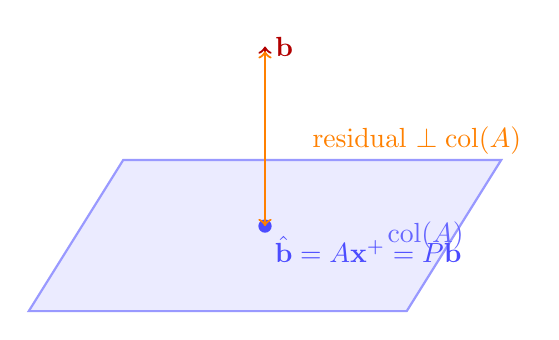
\begin{tikzpicture}[scale=1.2]
    \draw[thick, blue!40, fill=blue!8] (-2,-0.8) -- (2,-0.8) -- (3,0.8) -- (-1,0.8) -- cycle;
    \node[blue!60] at (2.2,0) {$\text{col}(A)$};
    \coordinate (bhat) at (0.5, 0.1);
    \coordinate (b) at (0.5, 2.0);
    \draw[thick, ->, red!70!black] (bhat) -- (b) node[right] {$\mathbf{b}$};
    \draw[thick, dashed, gray] (bhat) -- (b);
    \fill[blue!70] (bhat) circle (2pt) node[below right] {$\hat{\mathbf{b}} = A\mathbf{x}^+ = P\mathbf{b}$};
    \draw[thick, <->, orange] (0.5,0.1) -- (0.5, 1.95);
    \node[orange, right] at (0.9, 1.0) {residual $\perp \text{col}(A)$};
\end{tikzpicture}
\end{center}

The closest point $\hat{\mathbf{b}} \in \text{col}(A)$ to $\mathbf{b}$ is its \textbf{orthogonal projection} $\hat{\mathbf{b}} = P\mathbf{b}$, where $P$ is the orthogonal projector onto $\text{col}(A)$. The residual $\mathbf{b} - \hat{\mathbf{b}}$ is perpendicular to every column of $A$:
\[
    A^\top(\mathbf{b} - A\mathbf{x}^+) = \mathbf{0} \quad \Longleftrightarrow \quad A^\top A \mathbf{x}^+ = A^\top \mathbf{b}
\]
which is exactly the normal equations again — the geometric and calculus views are equivalent.

\textbf{The projection matrix.} The projector onto $\text{col}(A)$ is:
\[
    P = A(A^\top A)^{-1} A^\top
\]
and satisfies $P^2 = P$ (idempotent) and $P^\top = P$ (symmetric). Since $P = AA^+$, we read off:
\[
    A^+ = (A^\top A)^{-1} A^\top
\]

\begin{keybox}
\textbf{Key identity:} $AA^+$ is the orthogonal projector onto the \textbf{column space} of $A$. \\
\textbf{Key identity:} $A^+A$ is the orthogonal projector onto the \textbf{row space} of $A$.
\end{keybox}

Read together, the two identities say that $A^+$ inverts $A$ \emph{exactly where inversion is possible}: $A$ maps $\text{row}(A)$ bijectively onto $\text{col}(A)$, $A^+$ is the inverse of that bijection, and $A^+$ sends the leftover directions $\text{null}(A^\top) = \text{col}(A)^\perp$ to zero.

\subsection{Derivation 3: Tikhonov Regularisation (Limit)}

Add a regularisation term and solve:
\[
    \min_{\mathbf{x}}\; \|A\mathbf{x} - \mathbf{b}\|^2 + \lambda\|\mathbf{x}\|^2, \quad \lambda > 0
\]
The unique closed-form solution is:
\[
    \mathbf{x}_\lambda = (A^\top A + \lambda I)^{-1} A^\top \mathbf{b}
\]
$(A^\top A + \lambda I)$ is always invertible for $\lambda > 0$, even when $A^\top A$ is singular. The pseudoinverse emerges as the limit:
\[
    A^+ = \lim_{\lambda \to 0^+} (A^\top A + \lambda I)^{-1} A^\top
\]

The SVD makes this limit transparent. Substituting $A = U\Sigma V^\top$ diagonalises the problem:
\[
    \mathbf{x}_\lambda = \sum_{i=1}^{r} \underbrace{\frac{\sigma_i}{\sigma_i^2 + \lambda}}_{\text{filter factor}} (\mathbf{u}_i^\top \mathbf{b})\, \mathbf{v}_i,
    \qquad
    \frac{\sigma_i}{\sigma_i^2 + \lambda} \;\longrightarrow\; \frac{1}{\sigma_i} \quad \text{as } \lambda \to 0^+.
\]
Directions with $\sigma_i = 0$ never enter the sum, so the limit is exactly $V\Sigma^+U^\top\mathbf{b}$ — meaning the limit argument works even when $A$ is rank-deficient and the closed form $(A^\top A)^{-1}A^\top$ does not exist. Note also that the filter factor damps the small-$\sigma_i$ directions most strongly: ridge regression is a \emph{smooth} version of the truncated SVD of Section~\ref{sec:rankdef}.

This connects $A^+$ directly to \textbf{ridge regression} in machine learning ($\lambda > 0$ controls regularisation), and shows the pseudoinverse is numerically approximable in a stable way.

% ─────────────────────────────────────────────
\section{Handling Rank Deficiency: Manual Removal vs.\ SVD}
\label{sec:rankdef}

When $A$ is not full rank, neither closed form survives: $A^\top A$ and $AA^\top$ are singular, so $(A^\top A)^{-1}A^\top$ and $A^\top(AA^\top)^{-1}$ are undefined. The SVD formula $V\Sigma^+U^\top$ is the only expression that still works — this section examines why it is also the \emph{right} thing to do.

\subsection{A Natural but Flawed Intuition}

Suppose $A \in \mathbb{R}^{m \times n}$ is tall but rank-deficient, with rank $r < n$. Some columns are
linearly dependent — they carry no new information. A natural idea is:

\begin{enumerate}
    \item Identify and \textbf{remove} the redundant (linearly dependent) columns.
    \item This yields a smaller matrix $\tilde{A} \in \mathbb{R}^{m \times r}$ of full column rank.
    \item Apply the left pseudoinverse: $\tilde{A}^+ = (\tilde{A}^\top \tilde{A})^{-1}\tilde{A}^\top$.
    \item Solve and map the solution back to the original coordinates.
\end{enumerate}

This approach is \emph{valid in spirit} — the rank-$r$ subspace is genuinely what matters. However,
it runs into serious practical difficulties.

\subsection{Why Manual Removal Fails in Practice}

\textbf{Problem 1: Which columns do you drop?}

In clean textbook examples, a column may be exactly twice another. In real data, no two columns are
ever \emph{exactly} dependent — they are only \emph{nearly} dependent due to measurement noise,
floating-point errors, or correlation. This makes the keep/drop decision inherently ambiguous:

\[
    \mathbf{a}_3 = 2\mathbf{a}_1 + \varepsilon, \quad \|\varepsilon\| \ll 1
\]

Is $\mathbf{a}_3$ redundant? The answer depends on $\varepsilon$ in a way that has no clean threshold.
A hard binary decision (keep or drop) is numerically fragile.

\textbf{Problem 2: You lose track of the original variables.}

After dropping columns, $\tilde{A}$ operates on a reduced set of unknowns
$\tilde{\mathbf{x}} \in \mathbb{R}^r$, not the original $\mathbf{x} \in \mathbb{R}^n$.
The solution $\tilde{\mathbf{x}}^+$ does not directly answer what the dropped unknowns should be.
Typically one assigns them the value zero by convention, but this is an arbitrary choice with no
optimality guarantee.

\textbf{Problem 3: Mapping back is ambiguous.}

Even after solving in the reduced space, reconstructing a full $\mathbf{x} \in \mathbb{R}^n$
requires an explicit bookkeeping of which columns were dropped and a decision about how to fill in
the missing entries. This is error-prone and not unique.

\subsection{What SVD Does Instead}

SVD performs the \emph{same conceptual step} — discarding redundant directions — but does so
\textbf{automatically, optimally, and in a coordinate system perfectly adapted to $A$}.

\medskip

\textbf{Step 1: Rotate into a new basis (via $V^\top$).}

Instead of working in the original column coordinates, SVD rotates into the basis of
\emph{right singular vectors}. In this rotated space, the directions are ordered by how much
variance / information they carry (the singular values $\sigma_1 \geq \cdots \geq \sigma_r > 0$).

\textbf{Step 2: Identify redundant directions (via $\Sigma$).}

The zero singular values \emph{exactly} identify the null-space directions — no ambiguous
thresholding required in the exact case:
\[
    \Sigma = \operatorname{diag}(\underbrace{\sigma_1, \ldots, \sigma_r}_{\text{keep}},\;
                                  \underbrace{0, \ldots, 0}_{\text{discard}})
\]

\textbf{Step 3: Invert only the kept directions (via $\Sigma^+$).}

\[
    \Sigma^+ = \operatorname{diag}\!\left(\frac{1}{\sigma_1}, \ldots, \frac{1}{\sigma_r},\;
                                           0, \ldots, 0\right)^\top
\]

Setting the reciprocals of zero singular values to zero (rather than $\infty$) is the mathematically
principled choice: it produces the minimum-norm solution among all least-squares minimisers.

\textbf{Step 4: Rotate back automatically (via $V$).}

Because $V$ is orthogonal, the rotation is trivially reversed. The solution is returned in the
\emph{original} coordinate space with no bookkeeping:
\[
    \mathbf{x}^+ = V\Sigma^+ U^\top \mathbf{b}
\]

\subsection{Side-by-Side Comparison}

\begin{center}
\small
\renewcommand{\arraystretch}{1.5}
\begin{tabular}{lll}
    \toprule
    \textbf{Step} & \textbf{Manual removal} & \textbf{SVD pseudoinverse} \\
    \midrule
    Find redundancy     & Inspect columns (fragile)          & Non-zero $\sigma_i$ (automatic) \\
    Handle near-dependency & Hard threshold (arbitrary)      & Soft via $\sigma_i \approx 0$ \\
    Discard redundancy  & Delete columns (loses variables)   & Set $1/\sigma_i = 0$ in $\Sigma^+$ \\
    Solve reduced system & In smaller $\tilde{\mathbf{x}}$ space & In rotated space via $U^\top$ \\
    Map back            & Assign zeros (arbitrary)           & $V$ rotates back automatically \\
    Optimality of result & Not guaranteed                    & Minimum norm, guaranteed \\
    \bottomrule
\end{tabular}
\end{center}

\begin{keybox}
\textbf{Takeaway.} The intuition of ``remove linearly dependent columns'' is correct, but executing it
manually requires arbitrary choices at every step. SVD realises the same idea automatically, in an
optimally adapted coordinate system, with a guaranteed minimum-norm result and no bookkeeping.
Manual removal is SVD done poorly; SVD is manual removal done perfectly.
\end{keybox}

\subsection{The Near-Rank-Deficient Case: Truncated SVD}

SVD also handles the practically important case where $A$ is \emph{not} exactly rank-deficient but
has very small singular values. A \textbf{truncated SVD} sets all $\sigma_i < \epsilon$ to zero
before inverting:
\[
    \sigma_i^+ = \begin{cases} 1/\sigma_i & \text{if } \sigma_i \geq \epsilon \\ 0 & \text{if } \sigma_i < \epsilon \end{cases}
\]
This is precisely the principled version of the ``remove near-dependent columns'' idea — and it is
numerically stable where manual removal is not.

% ─────────────────────────────────────────────
\section{Summary}

\begin{center}
\renewcommand{\arraystretch}{1.5}
\begin{tabular}{ll}
    \toprule
    \textbf{Derivation approach} & \textbf{Core perspective} \\
    \midrule
    Least squares (calculus)   & $A^+$ is an optimiser: minimise $\|A\mathbf{x}-\mathbf{b}\|^2$ \\
    SVD                        & $A^+$ is a structured inverse: $V\Sigma^+U^\top$ \\
    Moore--Penrose axioms       & $A^+$ is the unique solution to four algebraic conditions \\
    Projection geometry        & $AA^+$ projects $\mathbf{b}$ onto $\text{col}(A)$; $\mathbf{x}^+$ realises that projection \\
    Tikhonov regularisation    & $A^+$ is the limit of ridge regression as $\lambda \to 0$ \\
    \bottomrule
\end{tabular}
\end{center}

\begin{keybox}
\textbf{Unifying intuition.} The Moore--Penrose pseudoinverse always finds the ``most sensible'' solution to $A\mathbf{x} = \mathbf{b}$: when no solution exists it finds the \emph{best approximate} one; when infinitely many exist it finds the \emph{simplest} one; and via SVD it does all of this stably even when $A$ is rank-deficient.
\end{keybox}

% ─────────────────────────────────────────────
\appendix
\section{Proofs}
\label{app:proofs}

\begin{proof}[Proof of Theorem~\ref{thm:uniqueness} (Uniqueness)]
Suppose $B$ and $C$ both satisfy all four conditions. Then
\begin{align*}
    AB &= (AB)^\top = B^\top A^\top = B^\top (ACA)^\top \\
       &= (AB)^\top (AC)^\top = (AB)(AC) = (ABA)C = AC,
\end{align*}
using \eqref{eq:p3}, then \eqref{eq:p1} for $C$, then \eqref{eq:p3} again for both products, then \eqref{eq:p1} for $B$. The mirror-image argument with \eqref{eq:p4} gives $BA = CA$. Therefore
\[
    B = BAB = (CA)B = C(AB) = C(AC) = CAC = C. \qedhere
\]
\end{proof}

\begin{proof}[Proof of Theorem~\ref{thm:svd} (Pseudoinverse via SVD)]
Orthogonality does all the work: in every product, the inner factors $V^\top V$ and $U^\top U$ collapse to $I$. For condition \eqref{eq:p1},
\[
    A A^+ A = U\Sigma V^\top \, V\Sigma^+ U^\top \, U\Sigma V^\top = U(\Sigma\Sigma^+\Sigma)V^\top = U\Sigma V^\top = A,
\]
since $\Sigma\Sigma^+\Sigma = \Sigma$ holds entrywise: $\sigma_i \cdot \tfrac{1}{\sigma_i} \cdot \sigma_i = \sigma_i$ for $i \leq r$, and $0 \cdot 0 \cdot 0 = 0$ beyond. Condition \eqref{eq:p2} is the same computation with the roles of $\Sigma$ and $\Sigma^+$ swapped. For \eqref{eq:p3} and \eqref{eq:p4}, note $AA^+ = U(\Sigma\Sigma^+)U^\top$ and $A^+A = V(\Sigma^+\Sigma)V^\top$, where $\Sigma\Sigma^+$ and $\Sigma^+\Sigma$ are diagonal with entries $1$ (for $i \leq r$) and $0$ (beyond) — hence symmetric, and the sandwiches $UDU^\top$, $VDV^\top$ inherit the symmetry. By Theorem~\ref{thm:uniqueness}, this construction \emph{is} the pseudoinverse.
\end{proof}

\end{document}
